\section{Early stage researchers}
\label{esrs}
The 12 ESRs form the core of the network, with the training and partnerships providing a scaffold for the completion of their respective outcomes. These ESRs work with HEP and industry partners throughout the 3 years of their doctoral study.%\par
%Shortly after the commencement of the ESR positions, each ESR supervisor completed a Personal Career Development Plan with their ESR. This document details the 

\subsection{Structure of ESR positions}
\label{esr-structure}
Each ESR is enrolled as a doctoral student at a partner university for 3 years. This university is typically also the primary institution of the ESR (2 industry-centred ESR positions are enrolled at a university near to the respective industry partner). At the end of the period of doctoral study, each ESR will receive a doctorate in particle physics from their university of enrollment.\par
\begin{figure*}[h!]
    \centering
    % Use the relevant command for your figure-insertion program
    % to insert the figure file. See example above.
    % If not, use
    %\vspace*{5cm}       % Give the correct figure height in cm
    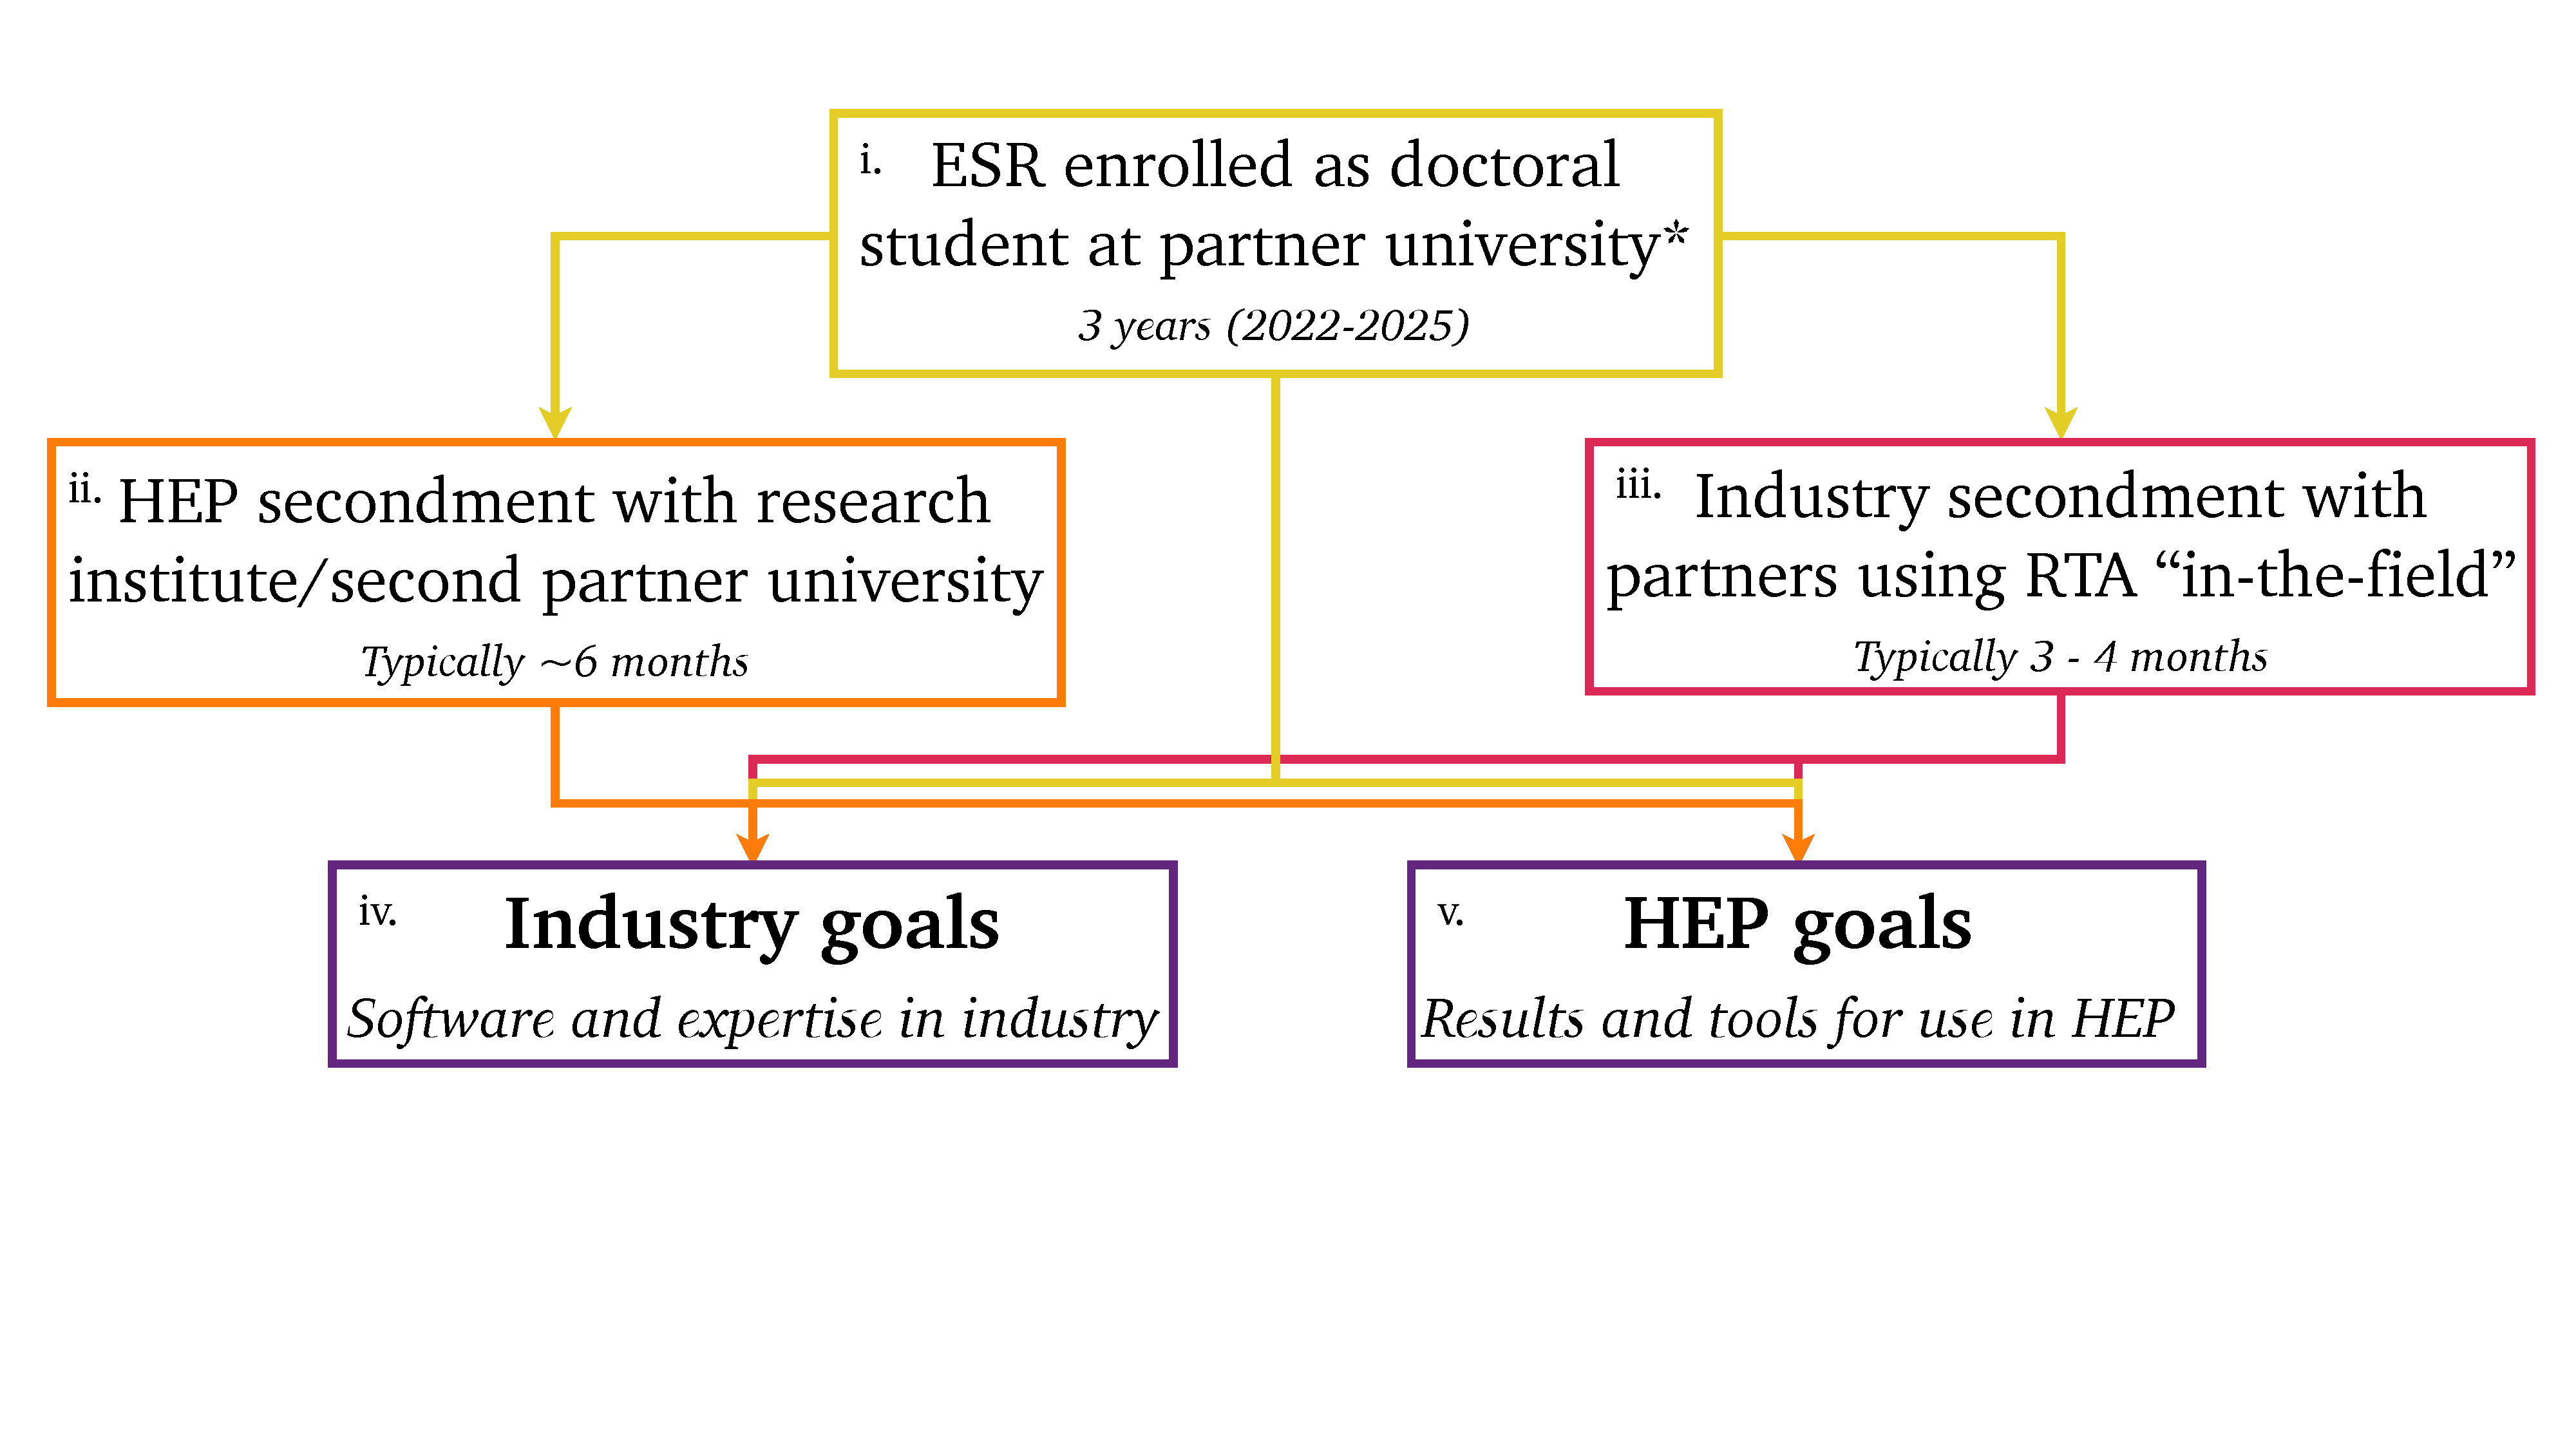
\includegraphics[width=0.9\linewidth,clip]{/Users/jgooding/Documents/SMARTHEP/CHEP2023/CHEP2023/proceedings/figures/esr-diagram.pdf}
    \caption{Diagram of the structure of a SMARTHEP ESR position. Each ESR is enrolled (i.). During the course of their enrolment, they will undertake secondments with network partners in HEP (ii.) and industry (iii.). Through the combination of their primary and secondment work, each ESR will achieve several goals in HEP (iv.) and industry (v.), as discussed in further detail in Section~\ref{goals}.}
    \label{esr-diagram}       % Give a unique label
\end{figure*}

Each ESR will undertake a secondment in HEP during their studies, either at another partner university or a partner research institute. This is generally organised to last for 6 months, though this varies from project to project.\par

In addition to their time working in HEP, each ESR will also spend time working in industry, typically as a secondment of 3-4 months (though this is again flexible to the specific programme of each ESR position).\par

To paint a clearer picture of how the positions take shape, a few examples are given. Jamie Gooding (ESR7) is based at Technische Universität Dortmund, working on real-time event selection at the LHCb Experiment, with a HEP secondment of $\approx 6$ months at CERN to support this work and a 3-4 month industry secondment with Ximantis, working on real-time traffic monitoring. Laura Boggia (ESR2)  \par